\section{System Overview} \label{sec:system_overview}

\begin{comment}

We introduce \textbf{AscendKernelGen}, a holistic \textbf{Generation-Evaluation Integrated} framework designed to automate the lifecycle of Ascend NPU kernel development. AscendEngineer operates as an automated pipeline. As illustrated in Figure~\ref{fig:system_overview}, the architecture streamlines the process from operator specification input to kernel generation, and seamlessly transitions into rigorous validation, ultimately quantifying model capabilities through multi-dimensional metrics.

The framework is composed of two synergistic sub-systems: the \textbf{Generation Sub-system} and the \textbf{Evaluation Sub-system}.

\paragraph{The Generation Sub-system.} This module addresses the scarcity of NPU-specific programming expertise and serves as the kernel production engine. It is built upon two core pillars: \begin{enumerate} \item \textbf{AscendC-Specific Corpus Construction:} We aggregate a comprehensive dataset from diverse high-quality sources, including the official Huawei CANN-ops library, the community-driven Catlass repository, and official documentation. Through rigorous cleaning and formatting, we construct a specialized instruction-tuning corpus tailored for the NPU hardware abstraction. \item \textbf{LLM Fine-Tuning for NPU Kernels:} Leveraging this corpus, we perform full-parameter fine-tuning on foundational models (e.g., Qwen 3) to align them with the complex AscendC programming paradigm. This process specifically targets the unique challenges of hardware-specific programming, such as optimizing memory tiling strategies, leveraging specialized compute units (e.g., SIMD Vector and Matrix Cube cores), and managing asynchronous computation pipelines. \end{enumerate}

\paragraph{The Evaluation Sub-system.} Acting as the verification engine, this sub-system systematically measures the quality of the generated kernels. It is designed to bridge the "API Gap" between probabilistic model outputs and deterministic hardware requirements: \begin{enumerate} \item \textbf{Hierarchical Task Definition:} We define a benchmark suite categorized into three difficulty levels. The representative operators were strategically selected to comprehensively cover diverse Compute-bound and Memory-bound workloads, as well as varying degrees of API usage complexity. Ranging from fundamental element-wise operations (L1) to complex operators like FlashAttention (L3), this suite evaluates the model's generalization capabilities across different computational patterns. \item \textbf{Multi-Stage Metrics:} The evaluation pipeline implements a strict filtering mechanism. It prioritizes \textit{Compilation Success} as the prerequisite, followed by \textit{Functional Correctness} verification against golden references (e.g., PyTorch). While the current iteration focuses on functional validity, the architecture allows for future extensibility into hardware performance metrics (e.g., latency, throughput) and deep static analysis of code quality (e.g., API hallucination rates and vectorization efficiency). \end{enumerate}

The following subsections detail the implementation of these components, starting with the data-centric generation approach.

\end{comment}

We present \textbf{AscendKernelGen (AKGen)}, a unified research framework for studying Large Language Model (LLM)-based generation of low-level NPU kernels. Rather than serving as a standalone engineering system, AKGen is designed to support systematic investigation of kernel generation, verification, and evaluation under realistic hardware programming constraints.

As illustrated in Fig.~\ref{fig:framework}, AKGen integrates three tightly coupled components: a domain-specific reasoning dataset, a kernel generation model, and a structured evaluation benchmark. Together, they form a closed generation--evaluation loop that enables controlled analysis of model capabilities and limitations.

\begin{figure*}[t]
    \centering
    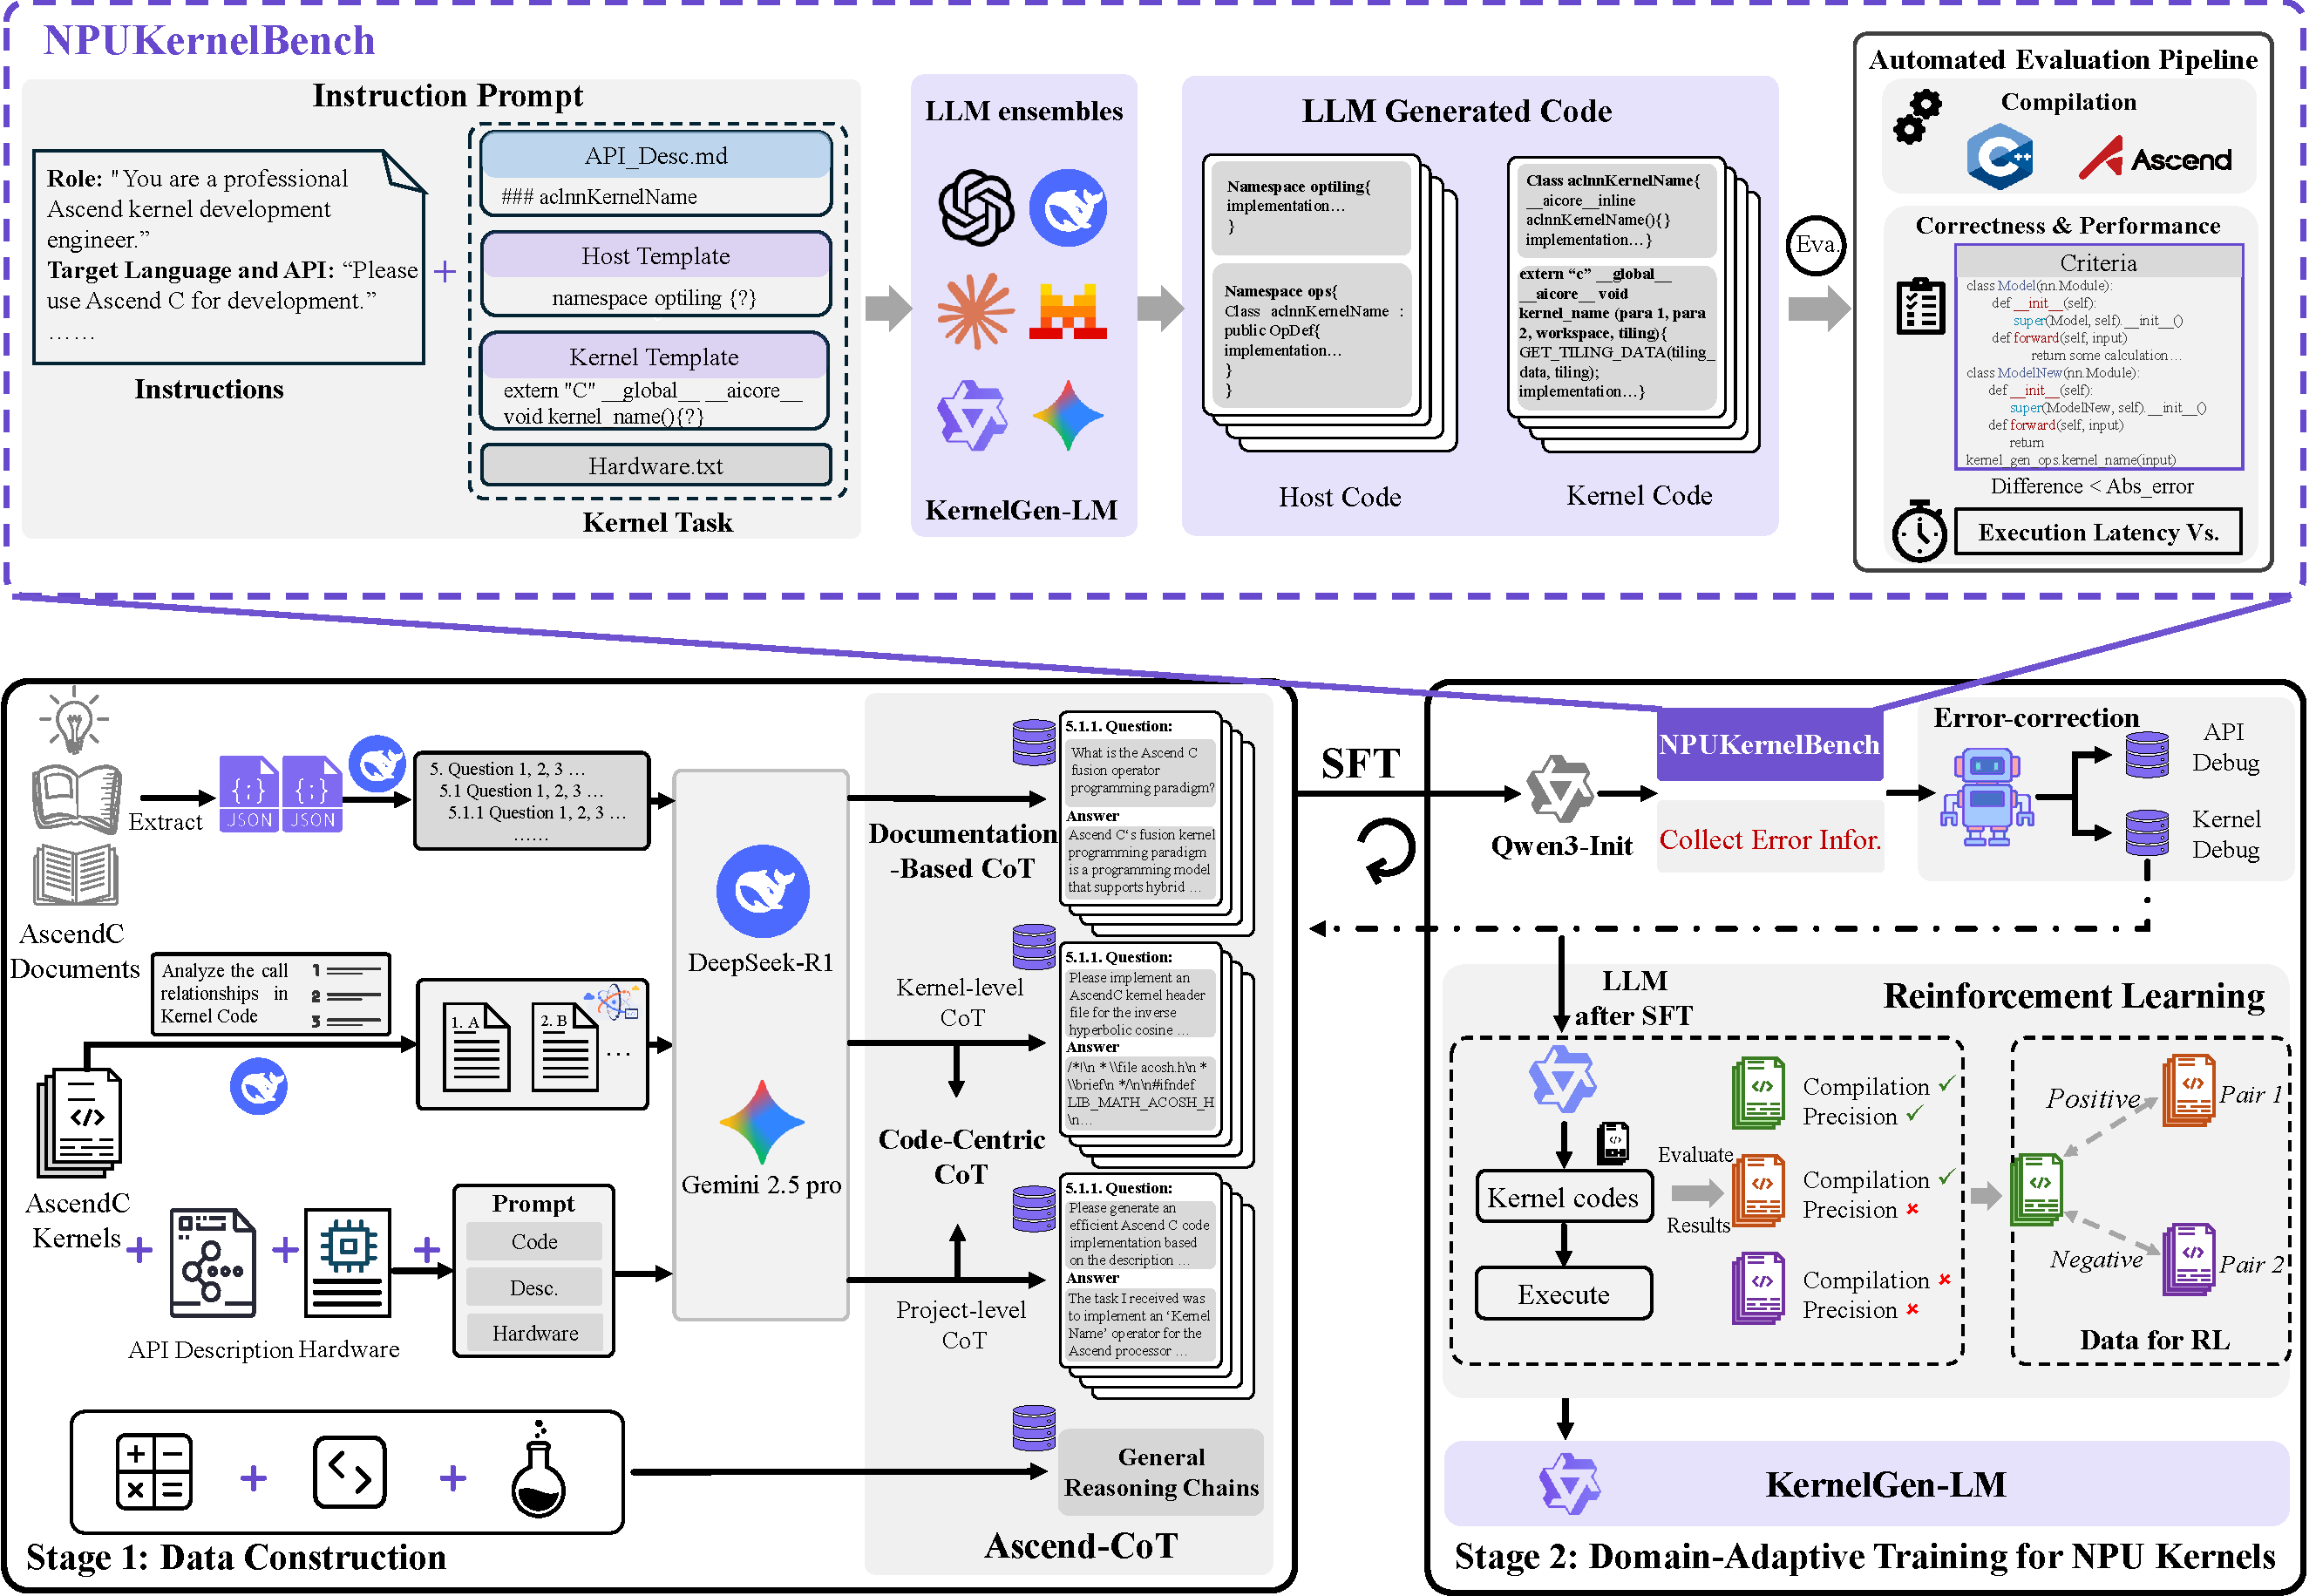
\includegraphics[width=1\linewidth]{pdfs/framework.pdf}
    \caption{System overview of AscendKernelGen, depicting the data construction, LLM training, and hardware-grounded evaluation pipeline for NPU kernel generation.}
    \label{fig:framework}
\end{figure*}

\paragraph{Generation Component.}
The generation side of AKGen is built upon two elements.

\begin{itemize}
    \item \textbf{Ascend Chain-of-Thought Dataset (Ascend-CoT).}
    To address the scarcity of low-level NPU programming data, we construct Ascend-CoT, a curated dataset that captures the structured reasoning processes required for AscendC kernel development. The dataset is collected from real-world operator implementations and documentation, and emphasizes explicit pipeline construction, synchronization logic, and arithmetic reasoning patterns essential to kernel correctness.

    \item \textbf{KernelGen-LM.}
    Using Ascend-CoT, we perform domain-adaptive post-training on a strong base LLM to obtain \textit{KernelGen-LM}, a model specialized for low-level NPU kernel generation. The training objective explicitly targets the reasoning challenges of hardware-aware code generation, including data tiling, asynchronous pipeline orchestration, and correct use of low-level programming interfaces.
\end{itemize}

\begin{comment}

\paragraph{Evaluation Component.}
To systematically assess generated kernels, AKGen incorporates a dedicated evaluation framework, \textit{NPUKernelBench}, which bridges the gap between probabilistic model outputs and deterministic hardware execution.

\begin{itemize}
    \item \textbf{Task Stratification.}
    NPUKernelBench organizes evaluation tasks into multiple difficulty levels, ranging from simple element-wise operators to complex fused kernels. This stratification enables fine-grained analysis of model behavior across diverse computational patterns and levels of programming complexity.

    \item \textbf{Multi-Stage Validation Metrics.}
    Each generated kernel is evaluated through a staged pipeline that checks compilation success, verifies functional correctness against reference implementations, and measures execution performance in terms of runtime. This design isolates distinct failure modes and allows us to quantify model performance beyond surface-level code validity. While the current study emphasizes correctness and performance metrics, the framework is readily extensible to additional analyses such as static code quality and deeper performance characterization.
\end{itemize}

\end{comment}

\paragraph{Evaluation Component.}
To systematically assess generated kernels, AKGen incorporates a dedicated evaluation framework, \textit{NPUKernelBench}, which bridges the gap between probabilistic model outputs and deterministic hardware execution. NPUKernelBench organizes evaluation tasks into multiple difficulty levels, ranging from simple element-wise operators to complex fused kernels, enabling fine-grained analysis of model behavior across diverse computational patterns and levels of programming complexity.

Each generated kernel is evaluated through a staged validation pipeline that checks compilation success, verifies functional correctness against reference implementations, and measures execution performance in terms of runtime. This multi-stage design isolates distinct failure modes and allows us to quantify model behavior beyond surface-level code validity. While the current study emphasizes correctness and performance metrics, the framework is readily extensible to additional analyses, such as static code quality assessment and deeper performance characterization.

Overall, AKGen provides a controlled framework for analyzing how LLMs acquire, apply, and generalize low-level hardware programming knowledge, with Ascend NPU kernels serving as a representative and challenging testbed.
